\documentclass{standalone}
\usepackage{tikz}
\usetikzlibrary{patterns, positioning}
\usepackage[sfdefault]{ClearSans} %% option 'sfdefault' activates Clear Sans as the default text font
\usepackage[T1]{fontenc}

\begin{document}
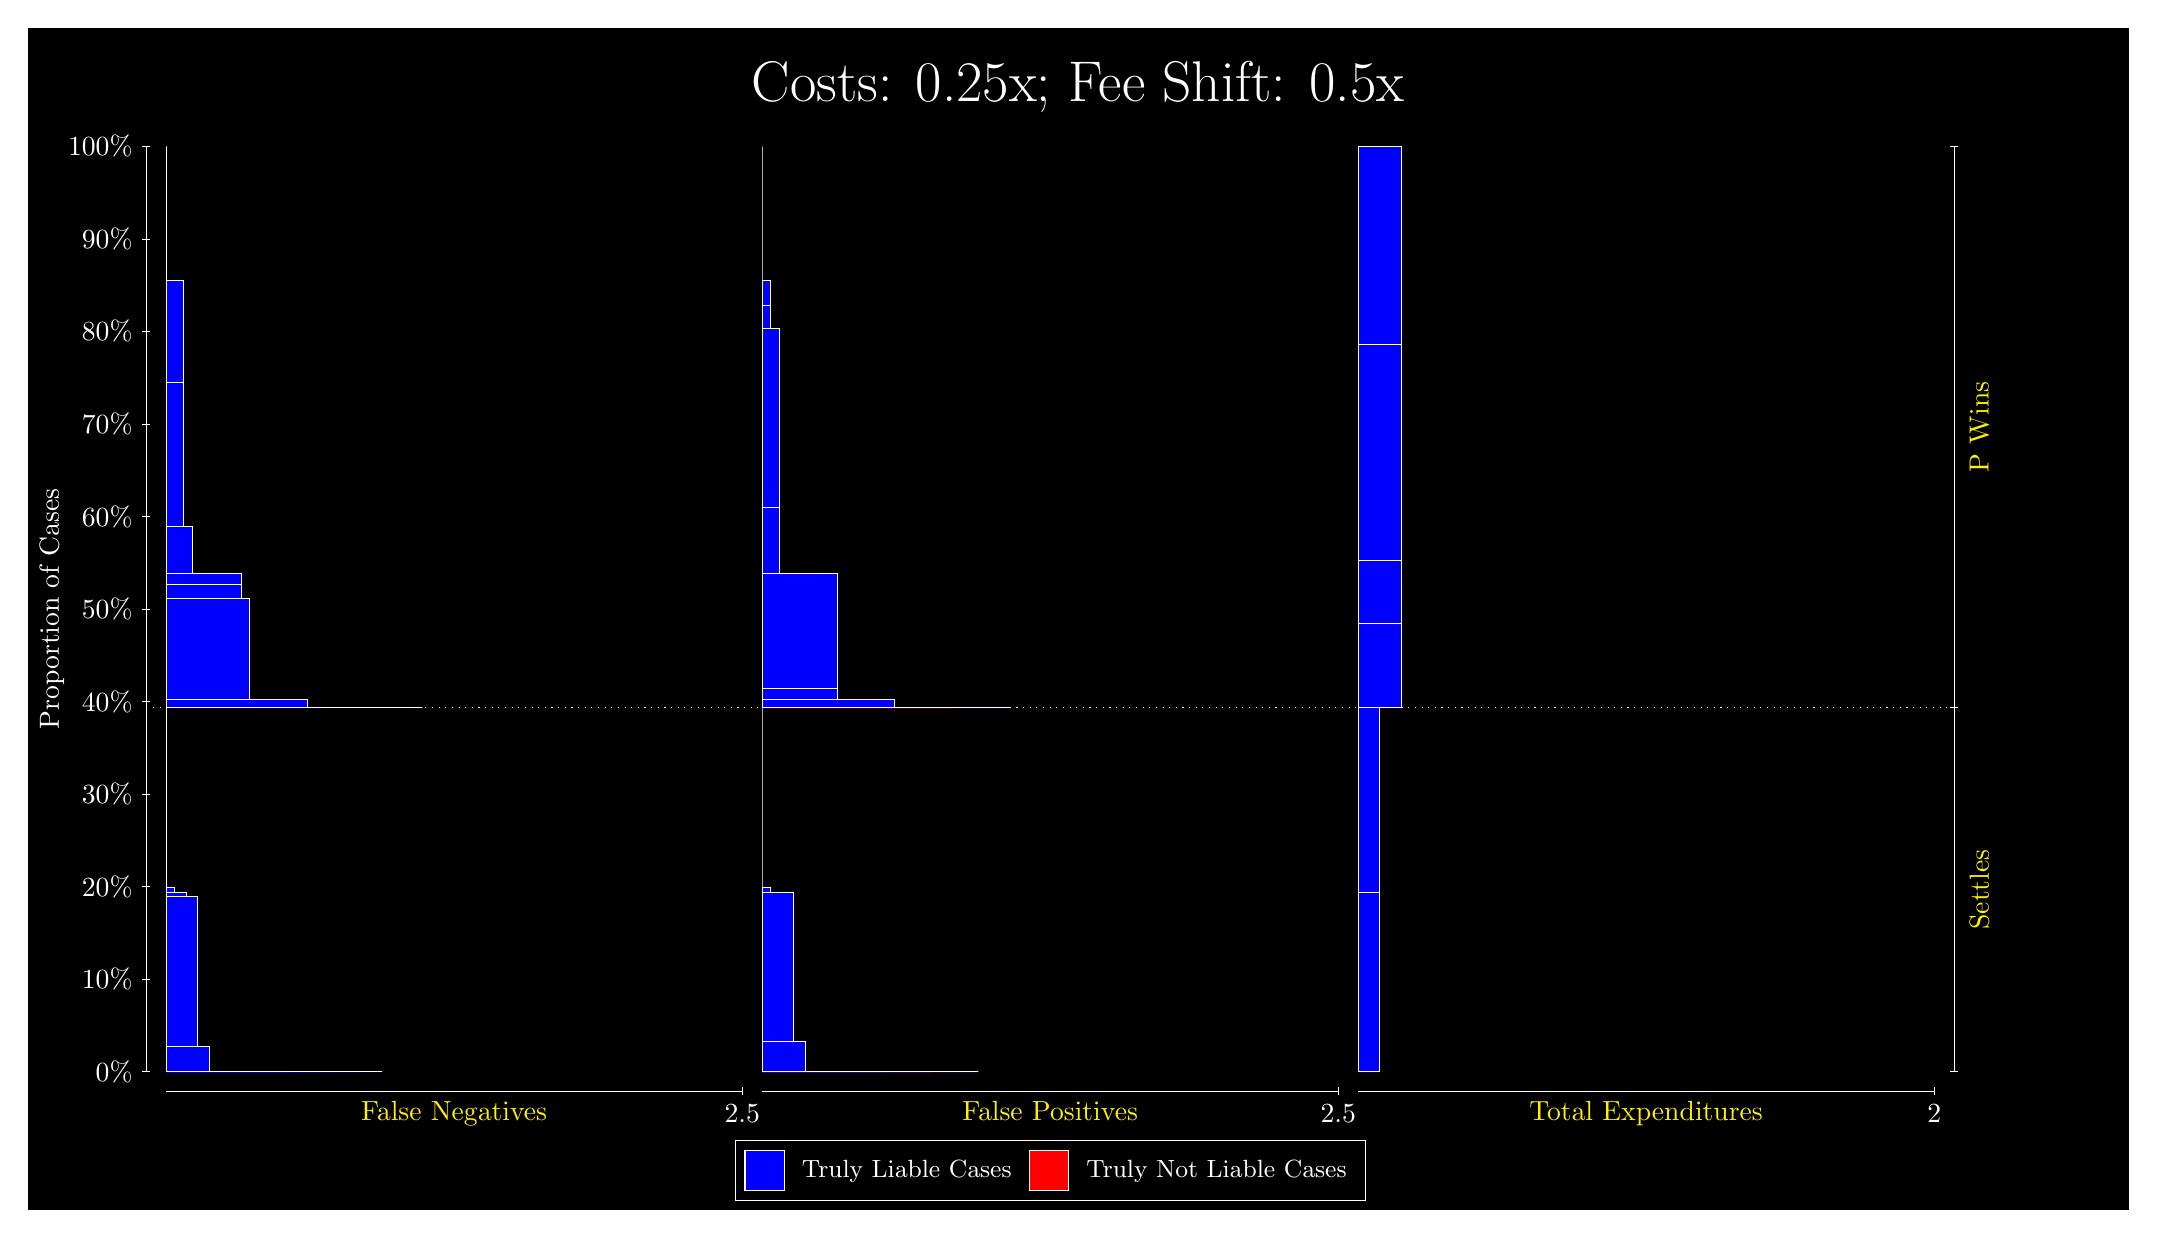
\begin{tikzpicture}
\draw[fill=black] (0,0) rectangle (26.667,15);
\draw[text=white] (0,13.5) rectangle (26.667,15) node[midway] {\huge Costs: 0.25x; Fee Shift: 0.5x};
\draw[white, very thin] (1.5,1.75) -- (1.5,13.5);
\node[rotate=90, text=white, anchor=center] at (0.3, 7.625) {Proportion of Cases};
\draw[white, very thin] (1.45,1.75) -- (1.55,1.75);
\node[text=white, anchor=east] at (1.45, 1.75) {0\%};
\draw[white, very thin] (1.45,2.925) -- (1.55,2.925);
\node[text=white, anchor=east] at (1.45, 2.925) {10\%};
\draw[white, very thin] (1.45,4.1) -- (1.55,4.1);
\node[text=white, anchor=east] at (1.45, 4.1) {20\%};
\draw[white, very thin] (1.45,5.275) -- (1.55,5.275);
\node[text=white, anchor=east] at (1.45, 5.275) {30\%};
\draw[white, very thin] (1.45,6.45) -- (1.55,6.45);
\node[text=white, anchor=east] at (1.45, 6.45) {40\%};
\draw[white, very thin] (1.45,7.625) -- (1.55,7.625);
\node[text=white, anchor=east] at (1.45, 7.625) {50\%};
\draw[white, very thin] (1.45,8.8) -- (1.55,8.8);
\node[text=white, anchor=east] at (1.45, 8.8) {60\%};
\draw[white, very thin] (1.45,9.975) -- (1.55,9.975);
\node[text=white, anchor=east] at (1.45, 9.975) {70\%};
\draw[white, very thin] (1.45,11.15) -- (1.55,11.15);
\node[text=white, anchor=east] at (1.45, 11.15) {80\%};
\draw[white, very thin] (1.45,12.325) -- (1.55,12.325);
\node[text=white, anchor=east] at (1.45, 12.325) {90\%};
\draw[white, very thin] (1.45,13.5) -- (1.55,13.5);
\node[text=white, anchor=east] at (1.45, 13.5) {100\%};

\draw[white, very thin] (24.457,1.75) -- (24.457,13.5);
\draw[white, very thin] (24.407,1.75) -- (24.507,1.75);
\node[anchor=west] at (24.407, 1.75) {};
\draw[white, very thin] (24.407,6.3729) -- (24.507,6.3729);
\node[anchor=west] at (24.407, 6.3729) {};
\draw[white, very thin] (24.407,13.5) -- (24.507,13.5);
\node[anchor=west] at (24.407, 13.5) {};

\draw[white, very thin, fill=blue] (1.75,1.75) rectangle (4.4946,1.75);
\draw[white, very thin, fill=blue] (1.75,1.75) rectangle (4.2018,1.75);
\draw[white, very thin, fill=blue] (1.75,1.75) rectangle (3.9091,1.75);
\draw[white, very thin, fill=blue] (1.75,1.75) rectangle (3.7627,1.75);
\draw[white, very thin, fill=blue] (1.75,1.75) rectangle (3.4699,1.75);
\draw[white, very thin, fill=blue] (1.75,1.75) rectangle (3.3236,1.75);
\draw[white, very thin, fill=blue] (1.75,1.75) rectangle (3.1772,1.75);
\draw[white, very thin, fill=blue] (1.75,1.75) rectangle (3.0308,1.7505);
\draw[white, very thin, fill=blue] (1.75,1.7505) rectangle (2.738,1.7527);
\draw[white, very thin, fill=blue] (1.75,1.7527) rectangle (2.5917,1.7548);
\draw[white, very thin, fill=blue] (1.75,1.7548) rectangle (2.4453,1.7553);
\draw[white, very thin, fill=blue] (1.75,1.7553) rectangle (2.2989,2.0667);
\draw[white, very thin, fill=blue] (1.75,2.0667) rectangle (2.1525,3.9735);
\draw[white, very thin, fill=blue] (1.75,3.9735) rectangle (2.0062,3.974);
\draw[white, very thin, fill=blue] (1.75,3.974) rectangle (2.0062,4.0323);
\draw[white, very thin, fill=blue] (1.75,4.0323) rectangle (1.8598,4.0905);
\draw[white, very thin, fill=red] (1.75,4.0905) rectangle (1.75,4.0905);
\draw[white, very thin, fill=blue] (1.75,4.0905) rectangle (1.75,6.3729);
\draw[white, very thin, fill=blue] (1.75,6.3729) rectangle (5.0069,6.3729);
\draw[white, very thin, fill=blue] (1.75,6.3729) rectangle (4.275,6.374);
\draw[white, very thin, fill=blue] (1.75,6.374) rectangle (4.1652,6.374);
\draw[white, very thin, fill=blue] (1.75,6.374) rectangle (3.5431,6.4833);
\draw[white, very thin, fill=blue] (1.75,6.4833) rectangle (3.4333,6.4834);
\draw[white, very thin, fill=blue] (1.75,6.4834) rectangle (2.8112,7.7655);
\draw[white, very thin, fill=blue] (1.75,7.7655) rectangle (2.7015,7.9388);
\draw[white, very thin, fill=blue] (1.75,7.9388) rectangle (2.7015,8.075);
\draw[white, very thin, fill=blue] (1.75,8.075) rectangle (2.0793,8.6808);
\draw[white, very thin, fill=blue] (1.75,8.6808) rectangle (1.9696,10.503);
\draw[white, very thin, fill=blue] (1.75,10.503) rectangle (1.9696,11.798);
\draw[white, very thin, fill=red] (1.75,11.798) rectangle (1.75,11.798);
\draw[white, very thin, fill=blue] (1.75,11.798) rectangle (1.75,13.5);
\draw[white, very thin, fill=red] (9.3189,1.75) rectangle (12.063,1.75);
\draw[white, very thin, fill=blue] (9.3189,1.75) rectangle (12.063,1.75);
\draw[white, very thin, fill=red] (9.3189,1.75) rectangle (11.478,1.75);
\draw[white, very thin, fill=blue] (9.3189,1.75) rectangle (11.478,1.75);
\draw[white, very thin, fill=blue] (9.3189,1.75) rectangle (11.332,1.75);
\draw[white, very thin, fill=red] (9.3189,1.75) rectangle (10.892,1.75);
\draw[white, very thin, fill=blue] (9.3189,1.75) rectangle (10.892,1.75);
\draw[white, very thin, fill=blue] (9.3189,1.75) rectangle (10.746,1.75);
\draw[white, very thin, fill=blue] (9.3189,1.75) rectangle (10.6,1.7527);
\draw[white, very thin, fill=red] (9.3189,1.7527) rectangle (10.307,1.7527);
\draw[white, very thin, fill=blue] (9.3189,1.7527) rectangle (10.307,1.7527);
\draw[white, very thin, fill=blue] (9.3189,1.7527) rectangle (10.161,1.7548);
\draw[white, very thin, fill=red] (9.3189,1.7548) rectangle (10.014,1.7548);
\draw[white, very thin, fill=blue] (9.3189,1.7548) rectangle (10.014,1.7579);
\draw[white, very thin, fill=blue] (9.3189,1.7579) rectangle (10.014,1.7584);
\draw[white, very thin, fill=blue] (9.3189,1.7584) rectangle (9.8678,2.1281);
\draw[white, very thin, fill=red] (9.3189,2.1281) rectangle (9.7214,2.1281);
\draw[white, very thin, fill=blue] (9.3189,2.1281) rectangle (9.7214,4.0319);
\draw[white, very thin, fill=blue] (9.3189,4.0319) rectangle (9.575,4.0324);
\draw[white, very thin, fill=blue] (9.3189,4.0324) rectangle (9.4287,4.0906);
\draw[white, very thin, fill=blue] (9.3189,4.0906) rectangle (9.3189,6.3729);
\draw[white, very thin, fill=red] (9.3189,6.3729) rectangle (12.466,6.3729);
\draw[white, very thin, fill=blue] (9.3189,6.3729) rectangle (12.466,6.3729);
\draw[white, very thin, fill=red] (9.3189,6.3729) rectangle (11.734,6.3729);
\draw[white, very thin, fill=blue] (9.3189,6.3729) rectangle (11.734,6.374);
\draw[white, very thin, fill=red] (9.3189,6.374) rectangle (11.002,6.374);
\draw[white, very thin, fill=blue] (9.3189,6.374) rectangle (11.002,6.4834);
\draw[white, very thin, fill=red] (9.3189,6.4834) rectangle (10.892,6.4834);
\draw[white, very thin, fill=blue] (9.3189,6.4834) rectangle (10.892,6.4834);
\draw[white, very thin, fill=red] (9.3189,6.4834) rectangle (10.27,6.4834);
\draw[white, very thin, fill=blue] (9.3189,6.4834) rectangle (10.27,6.6194);
\draw[white, very thin, fill=blue] (9.3189,6.6194) rectangle (10.27,8.0747);
\draw[white, very thin, fill=red] (9.3189,8.0747) rectangle (10.161,8.0747);
\draw[white, very thin, fill=blue] (9.3189,8.0747) rectangle (10.161,8.075);
\draw[white, very thin, fill=blue] (9.3189,8.075) rectangle (9.5384,8.9186);
\draw[white, very thin, fill=blue] (9.3189,8.9186) rectangle (9.5384,11.192);
\draw[white, very thin, fill=red] (9.3189,11.192) rectangle (9.4287,11.192);
\draw[white, very thin, fill=blue] (9.3189,11.192) rectangle (9.4287,11.486);
\draw[white, very thin, fill=blue] (9.3189,11.486) rectangle (9.4287,11.798);
\draw[white, very thin, fill=blue] (9.3189,11.798) rectangle (9.3189,13.5);
\draw[white, very thin, fill=red] (16.888,1.75) rectangle (17.162,1.75);
\draw[white, very thin, fill=blue] (16.888,1.75) rectangle (17.162,4.0292);
\draw[white, very thin, fill=red] (16.888,4.0292) rectangle (17.162,4.0292);
\draw[white, very thin, fill=blue] (16.888,4.0292) rectangle (17.162,6.3729);
\draw[white, very thin, fill=red] (16.888,6.3729) rectangle (17.437,6.3729);
\draw[white, very thin, fill=blue] (16.888,6.3729) rectangle (17.437,7.4381);
\draw[white, very thin, fill=red] (16.888,7.4381) rectangle (17.437,7.4381);
\draw[white, very thin, fill=blue] (16.888,7.4381) rectangle (17.437,8.2484);
\draw[white, very thin, fill=red] (16.888,8.2484) rectangle (17.437,8.2484);
\draw[white, very thin, fill=blue] (16.888,8.2484) rectangle (17.437,10.981);
\draw[white, very thin, fill=red] (16.888,10.981) rectangle (17.437,10.981);
\draw[white, very thin, fill=blue] (16.888,10.981) rectangle (17.437,13.5);
\draw[white, dotted] (1.5,6.3729) -- (24.457,6.3729);
\draw[white, very thin] (1.75,1.5) -- (9.0689,1.5);
\node[text=yellow, anchor=north] at (5.4094, 1.5) {False Negatives};
\draw[white, very thin] (9.0689,1.45) -- (9.0689,1.55);
\node[text=white, anchor=north] at (9.0689, 1.45) {2.5};

\draw[white, very thin] (9.3189,1.5) -- (16.638,1.5);
\node[text=yellow, anchor=north] at (12.978, 1.5) {False Positives};
\draw[white, very thin] (16.638,1.45) -- (16.638,1.55);
\node[text=white, anchor=north] at (16.638, 1.45) {2.5};

\draw[white, very thin] (16.888,1.5) -- (24.207,1.5);
\node[text=yellow, anchor=north] at (20.547, 1.5) {Total Expenditures};
\draw[white, very thin] (24.207,1.45) -- (24.207,1.55);
\node[text=white, anchor=north] at (24.207, 1.45) {2};

\node[text=yellow, centered, rotate=90] at (24.777, 4.0614) {Settles};
\node[text=yellow, centered, rotate=90] at (24.777, 9.9364) {P Wins};

\draw (12.978300999999998,1.5) node[draw=none] (baseCoordinate) {};
\begin{scope}[align=center]
        \matrix[scale=0.5, draw=white, below=0.5cm of baseCoordinate, nodes={draw}, column sep=0.1cm]{
            \node[rectangle, draw, minimum width=0.5cm, minimum height=0.5cm, fill=blue] {}; &
            \node[draw=none, font=\small, text=white] (B) {Truly Liable Cases}; &
            \node[rectangle, draw, minimum width=0.5cm, minimum height=0.5cm, fill=red] {}; &
            \node[draw=none, font=\small, text=white] (B) {Truly Not Liable Cases}; \\
            };
\end{scope}

\end{tikzpicture}
\end{document}